\section{Thermodynamics}
The free energy\footnote{As we are in the grand canonical ensemble, this is the \emph{grand canonical} free energy, and not Helmholtz' free energy.}
is defined as
\begin{equation}
    \label{thermodynamic free energy}
    F = U - TS - \mu_I Q_I, \quad \dd F = - S \dd T - P \dd V - Q_I \dd \mu_I ,
\end{equation}
where $Q_I$ is the isospin charge, and $U$ is the energy.
As we have seen earlier, our system is homogenous.
This means that the free energy density is independent of volume, and thus $F = V \Ef$.
From  \cref{thermodynamic free energy} we see that the pressure is given by
\begin{equation}
    P = - \left(\diffp{F}{V}\right)_{T, \mu_I} = - \Ef.
\end{equation}
We are interested in the pressure relative to the state in which $\mu_I$ = 0. We therefore normalize $P(\mu_I=0) = 0$, which gives  
\begin{equation}
    P(\mu_I) = -(\Ef(\mu_I) - \Ef(\mu_I = 0))
\end{equation}
This is illustrated in \autoref{fig:pressure}.
\begin{figure}[h]
    \centering
    \vspace{-0.2cm}
    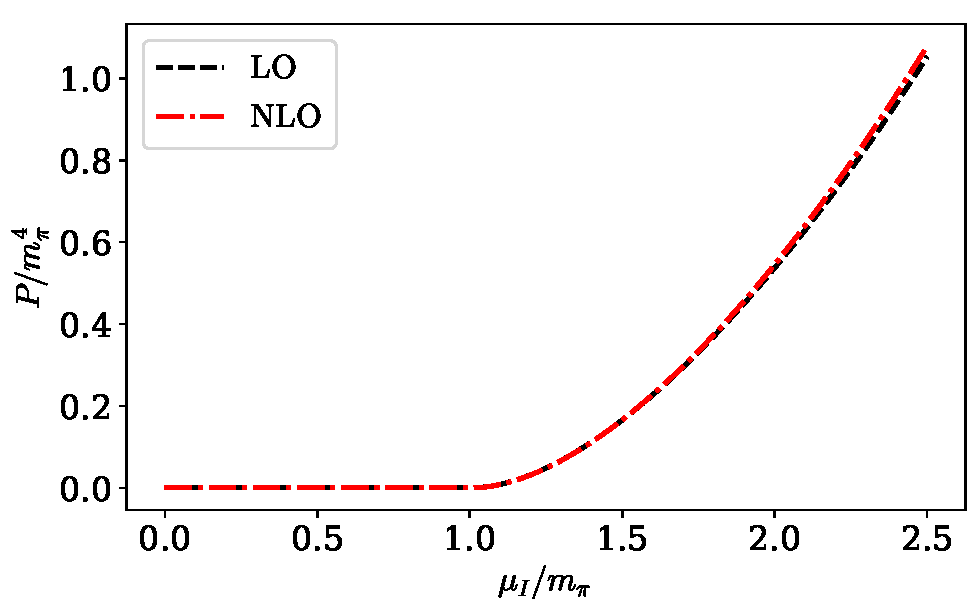
\includegraphics[width=0.7\textwidth]{figurer/numerics/pressure.pdf}
    \caption{The NLO and LO result for the pressure of the pions, as a function of $\mu_I$.}
    \label{fig:pressure}
\end{figure}

Likewise, the total isospin is proportional to volume, which means that the isospin density is
\begin{equation}
    n_I = \frac{Q_I}{V} = - \frac{1}{V} \left(\diffp{F}{\mu_I}\right)_{T, V}
    = - \diffp{\Ef}{\mu_I}.
\end{equation}
This gives 
\begin{align}
    \nonumber
    n_I & = 
    f^2 \mu_I \sin^2 \alpha
    - \diffp{\Ef_\mathrm{fin}}{\mu_I} \\
    & + \frac{1}{(4 \pi)^2}
    \left[
            \left(2\bar l_4+\ln\frac{M^2}{m_3^2}\right)\bar m^2 \mu_I \cos\alpha \sin^2 \alpha
            +\frac{1}{3}\left(2\bar l_1 + 4 \bar l_2 + 3\ln\frac{M^2}{m_3^2}\right)\mu_I^3 \sin^4 \alpha
    \right]
\end{align}
The isospin density, as a function of $\mu_I$, is shown in \autoref{fig:isospin_density}.
\begin{figure}[!h]
    \centering
    \vspace{-0.2cm}
    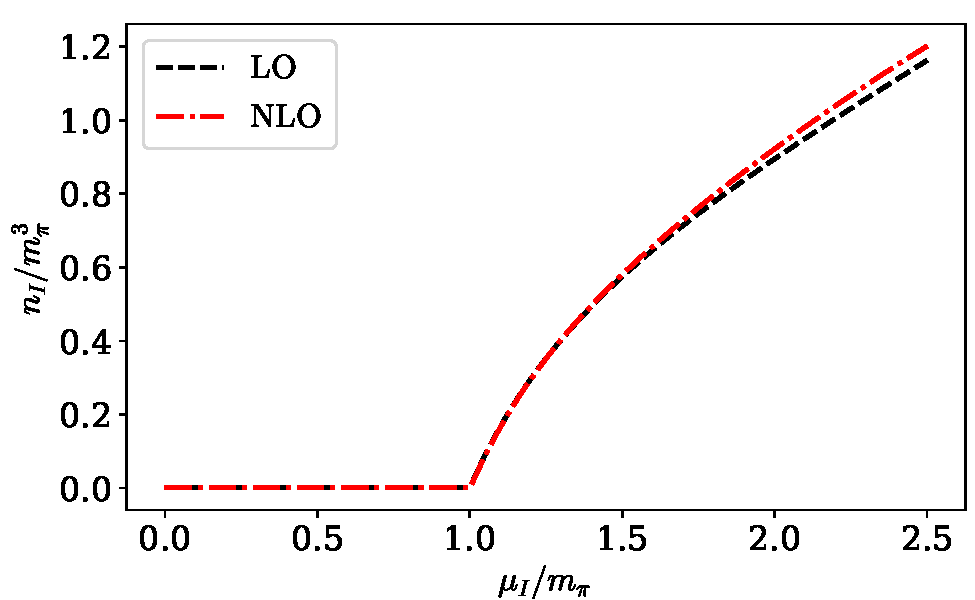
\includegraphics[width=0.7\textwidth]{figurer/numerics/isospin_density.pdf}
    \caption{The NLO and LO result for the isosopin densisty, as a function of $\mu_I$.}
    \label{fig:isospin_density}
\end{figure}

From \cref{thermodynamic free energy} we get the energy density, $u = U/V$ is given by
\begin{equation}
    u(\mu_I) = -P(\mu_I) + \mu_I n_I(\mu_I),
\end{equation}
where we again have normalized so that $u(\mu_I = 0) = 0$.
Now that we have both the dependence of pressure and energy density on the isospin chemical potential, we can trace out the line in the pressure-energy density plane, parametrized by $\mu_I$.
This is shown in \autoref{fig:equation of state}.
This line is the equation of state of the system.

\begin{figure}[!h]
    \centering
    \vspace{-0.2cm}
    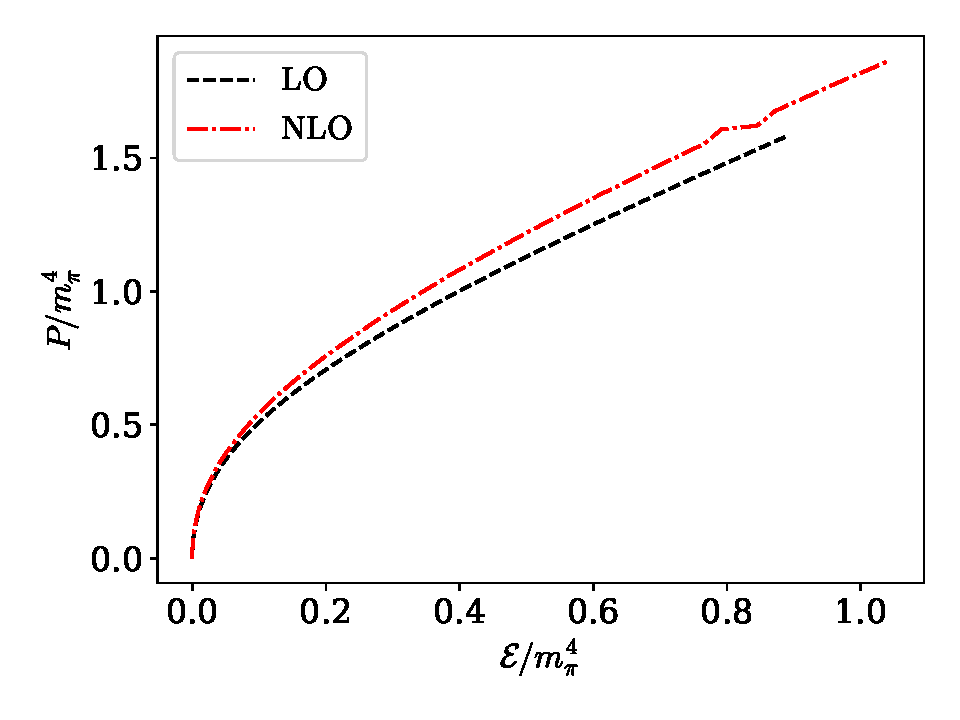
\includegraphics[width=0.7\textwidth]{figurer/numerics/energy_density.pdf}
    \caption{The equation of state of the pions.}
    \label{fig:equation of state}
\end{figure}

\FloatBarrier

\subsection*{Phase transition}
In our leading-order analysis, we saw that $\alpha$ was zero for $\mu_I \leq m_\pi$, before it starts to increase for $\mu_I>\alpha$, as shown in \autoref{fig:alpha}.
This is the hallmark of a phase transition, where $\alpha$ is the order parameter.
The transition is continuous in alpha, which means this is a second order phase transition.
Using \cref{leading order contribution free energy}, we can expand the leading-order free energy in $\alpha$,
\begin{align}
    \Ef_0^{(2)} 
    & = -f^2 \bar m^2 + f^2 \frac{1}{2}(\bar m^2 - \mu_I^2)\alpha^2
    +\frac{1}{24} f^2 (\bar m^2 - 4 \mu_I^2) \alpha^4 + \Oh[5]{\alpha} \\
    & = \Ef_0^{(2)}(\alpha=0) + a(\mu_I)\alpha^2 - \frac{1}{2} b(\mu_I)\alpha^4 + \Oh[5]{\alpha}.
\end{align}
Notice that near $\mu_I = \bar m$, $b > 0$.
As earlier, the equation that governs $\alpha$ is
\begin{equation}
    \label{landau ginsburg lo}
    \diffp{\Ef_0^{(2)}}{\alpha} = 2 [a(\mu_I) - b(\mu_I) \alpha^2] \alpha = 0.
\end{equation}
If $a<0$, then $\alpha = 0$ will be the only solution, which gives us the criterion for a phase transition 
\begin{equation}
    a(\mu_I) = 0,
\end{equation}
which again gives $\mu_I = \bar m$.
Near $\mu_I = \bar m$, we can write
\begin{equation}
    a = a_0 (\bar m - \mu_I), \quad b = b_0,
\end{equation}
so the solution to \cref{landau ginsburg lo} for $\mu_I>\bar m$
\begin{equation}
    \alpha(\mu_I) = \frac{a_0}{b_0} (\mu_I - \bar m)^{1/2}.
\end{equation}

In the vacuum phase, $\alpha = 0$, the ground state is given by 
\begin{equation}
    \Sigma(\pi = 0) = \one,
\end{equation}
where we have use \cref{sigma}.
$\Sigma$ transforms as (FORKLAR)
\begin{equation}
    \Sigma(x) \rightarrow \Sigma'(x) = V \Sigma(x) V^\dagger,
    \quad
    V = \exp{i \theta_a \tau_a}.
\end{equation}
which means that the vacuum phase ground state is invariant under $H$.
However, for $\alpha = 0$, the ground state is shifted to
\begin{equation}
    \Sigma(\pi=0) = \exp{i \alpha \tau_1}.
\end{equation}
The generators $\tau_2$ and $\tau_3$ are broken
